
\documentclass[crop,tikz]{standalone}
\usepackage[utf8]{inputenc}
\usepackage{tikz}
\usepackage{pgfplots}
\pgfplotsset{compat=newest}
\usepgfplotslibrary{groupplots}
\begin{document}
% This file was created by matplotlib2tikz v0.6.15.
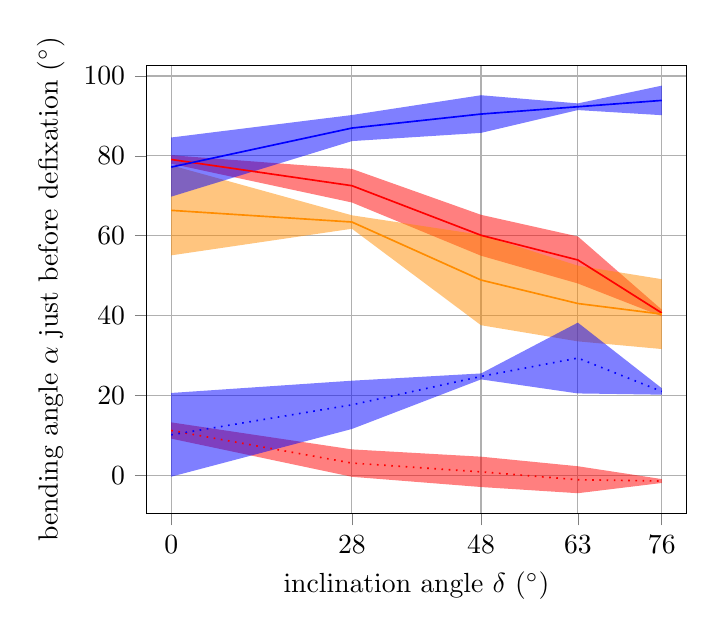
\begin{tikzpicture}

\definecolor{color0}{rgb}{1,0.549019607843137,0}

\begin{axis}[
xlabel={inclination angle $\delta$ ($^\circ$)},
ylabel={bending angle $\alpha$ just before defixation ($^\circ$)},
xmin=-3.8, xmax=79.8,
ymin=-9.60146301400235, ymax=102.682324660806,
tick align=outside,
tick pos=left,
xmajorgrids,
x grid style={lightgray!92.026143790849673!black},
ymajorgrids,
y grid style={lightgray!92.026143790849673!black},
xtick={0, 28, 48, 63, 76}
]
\path [fill=red, fill opacity=0.5] (axis cs:0,78.0253151942543)
--(axis cs:0,80.1503783820576)
--(axis cs:28,76.7238248858384)
--(axis cs:48,65.2253068496506)
--(axis cs:63,59.803628084364)
--(axis cs:76,41.4759293272738)
--(axis cs:76,39.8095658767124)
--(axis cs:76,39.8095658767124)
--(axis cs:63,48.0266635033117)
--(axis cs:48,54.9773674648634)
--(axis cs:28,68.3142234367075)
--(axis cs:0,78.0253151942543)
--cycle;

\path [fill=color0, fill opacity=0.5] (axis cs:0,55.0707827417364)
--(axis cs:0,77.6203064153689)
--(axis cs:28,65.1034327480933)
--(axis cs:48,60.2098665488505)
--(axis cs:63,52.4891627886378)
--(axis cs:76,49.1079341279603)
--(axis cs:76,31.6094297998251)
--(axis cs:76,31.6094297998251)
--(axis cs:63,33.534979441233)
--(axis cs:48,37.5762772580278)
--(axis cs:28,61.7381333062291)
--(axis cs:0,55.0707827417364)
--cycle;

\path [fill=blue, fill opacity=0.5] (axis cs:0,69.7738574195419)
--(axis cs:0,84.5898311406298)
--(axis cs:28,90.2203541261544)
--(axis cs:48,95.1768309076501)
--(axis cs:63,93.1302250712086)
--(axis cs:76,97.5785161301329)
--(axis cs:76,90.1789426528443)
--(axis cs:76,90.1789426528443)
--(axis cs:63,91.4610104191676)
--(axis cs:48,85.7509216496207)
--(axis cs:28,83.6918842198056)
--(axis cs:0,69.7738574195419)
--cycle;

\path [fill=red, fill opacity=0.5] (axis cs:0,9.17353647879756)
--(axis cs:0,13.244790017302)
--(axis cs:28,6.47909134248686)
--(axis cs:48,4.65076597472358)
--(axis cs:63,2.25428765547605)
--(axis cs:76,-0.961437525259766)
--(axis cs:76,-1.9363487891952)
--(axis cs:76,-1.9363487891952)
--(axis cs:63,-4.49765448332924)
--(axis cs:48,-2.94998487044941)
--(axis cs:28,-0.386124843313229)
--(axis cs:0,9.17353647879756)
--cycle;

\path [fill=blue, fill opacity=0.5] (axis cs:0,-0.355317569316513)
--(axis cs:0,20.6068441207131)
--(axis cs:28,23.6804935953736)
--(axis cs:48,25.4982735515773)
--(axis cs:63,38.222383389496)
--(axis cs:76,21.7940952976649)
--(axis cs:76,20.1834329901045)
--(axis cs:76,20.1834329901045)
--(axis cs:63,20.4911831279428)
--(axis cs:48,24.0120606702466)
--(axis cs:28,11.5938024172562)
--(axis cs:0,-0.355317569316513)
--cycle;

\addplot [semithick, red, forget plot]
table {%
0 79.0878467881559
28 72.5190241612729
48 60.101337157257
63 53.9151457938378
76 40.6427476019931
};
\addplot [semithick, color0, forget plot]
table {%
0 66.3455445785526
28 63.4207830271612
48 48.8930719034391
63 43.0120711149354
76 40.3586819638927
};
\addplot [semithick, blue, forget plot]
table {%
0 77.1818442800858
28 86.95611917298
48 90.4638762786354
63 92.2956177451881
76 93.8787293914886
};
\addplot [semithick, red, dotted, forget plot]
table {%
0 11.2091632480498
28 3.04648324958682
48 0.850390552137082
63 -1.1216834139266
76 -1.44889315722748
};
\addplot [semithick, blue, dotted, forget plot]
table {%
0 10.1257632756983
28 17.6371480063149
48 24.7551671109119
63 29.3567832587194
76 20.9887641438847
};
\end{axis}

\end{tikzpicture}
%% End matplotlib2tikz content %% 
\end{document}